\section{Model-View-Intent}
\label{sec:model-view-intent}
Model-View-Intent (MVI) ist eine weiteres Entfursmuster, welches der Feder von André (Medeiros) Staltz entstammt. Er stellte dieses auf einer Javascript Konferenz im Jahre 2015 vor
\cite{modelViewIntentIntroduction}. Es gehört damit zu den jüngsten seiner Art.
Seine ursprüngliche Anwendung fand es in dem ebenfalls von André Staltz geschaffenen Framework CycleJs, hat seit der Artikelreihe von Hannes Dorfmann in 2016
\cite{modelViewIntentOnAndroidHannesDorfmann2016}
aber auch den Sprung in die Welt von Android vollbracht. MVI bezieht den Großteil seines Design aus den hier bereits vorstellten Ideen und Konzepten. Das erste Ziel ist, ähnlich wie bei MVC, Informationen zwischen zwei Welten zu übersetzten: der des digitalen Bereichs des Computers und des mentalen Modells des Benutzers. Oder anders formuliert: Das Programm muss verstehen, was der Nutzer im Sinn hat.
Der zweite, zentrale Punkt von MVI besteht in der Handhabung des Zustands der Anwendung. Hierfür ist zu klären, was genau der Zustand inne hat.
\\
\\
MVI betrachtet dafür die Interaktion zwischen einem Nutzer und Programm als einen Kreis(lauf). Betätigt der Nutzer bswp. einen Knopf, sein Output, so gestaltet sich dieser als Input für das Programm. Dieses wiederum erzeugt einen Output (z.B. eine Meldung), welcher zum Input des Nutzers wird (hier: lesen).
\begin{figure}[ht]
	\centering
	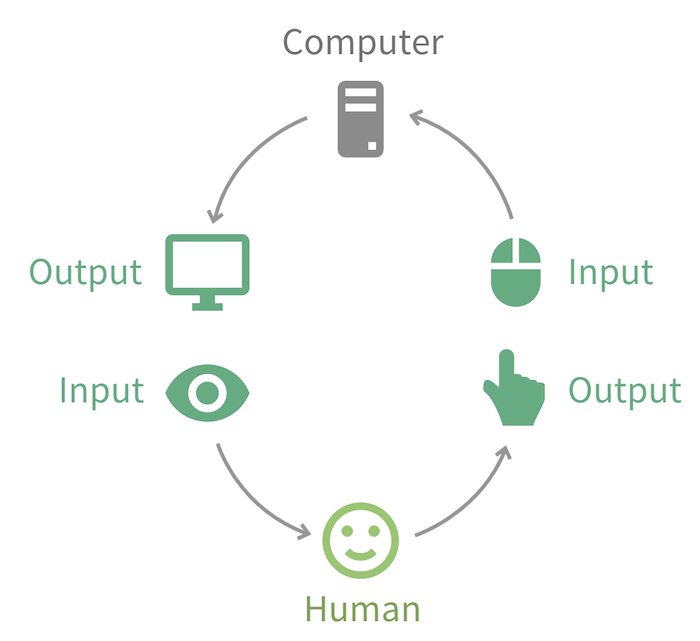
\includegraphics[height=0.5\textwidth]{./images/mvi-cycle}
	\caption{Nutzer und Computer als Input und Output}
	\caption*{Source: https://cycle.js.org/dialogue.html}
	\label{fig:userComputerInputOutput}
\end{figure}
\\
Die Grundprinzipien für den Aufbau der Architektur entspringen dabei dem beschriebenen, originalem Model-View-Controller. Das,
was MVC jedoch inkompatibel für die von MVI vorhergesehenen Prozesse macht, ist die Tatsache, das der Controller proaktiv ist. Dies bedeutet, dass der Controller selbstbestimmt über das Model und View verfügen und diese direkt manipulieren kann. Zwangsläufig wissen die jeweiligen Komponenten auch, von welchen Komponenten sie abhängig sind. Oder anders ausgedrückt: Eine Komponente deklariert, welche anderen Komponenten sie beeinflussen, anstatt dass andere Komponenten explizit aktualisiert werden (z.B. das Modell). Dabei wird das Prinzip des unidirektionale Datenfluss verletzt, welches auch in MVI strikt verfolgt wird. 
\\
\\
Um dieses unter anderem zu erreichen, setzt MVI zusätzlich auf Reaktive Programmierung. Für MVI bedeutet reaktiv zu sein, dass jede Komponente ihre Abhängigkeiten beobachtet und auf Veränderungen dieser reagiert. Die drei Komponenten werden durch Observables repräsentiert, wobei der Output jeweils der Input einer anderen Komponente ist.
\\
\\
Fast noch wichtiger als der reaktive Ansatz ist zu verstehen, wie der Kreislauf in Figur \ref{fig:datenflussFlux} programmatisch etabliert werden kann. Betrachtet man diesen Kreis etwas genauer, so wird deutlich, dass auf einen Input immer ein Output folgt. Dieses Konzept findet man auch in der Mathematik wieder: Funktionen. Mit diesen lässt sich MVI wie folgt illustrieren:
\\
\\
\textbf{Intent}: Das I in MVI steht für Intent und stellt den Teil da, welches es von den anderen Entwurfsmustern unterscheidet. Das Ziel der Intent-Fuktion ist es, die Absicht des Nutzer im digitalen Kontext des Programms auszudrücken.
Ein Ereignis (oder Event), z.B. die Eingabe eines Buchstaben, kann hier der Input sein.
Der Output dieser Funktion (z.B. ein String) wird zum Input der nächsten:
\\
\\
\textbf{Model}: Die Model-Funktion nimmt das entgegen, was die Intent-Funktion produziert. Ihre Aufgabe liegt in der Verwaltung des Zustands: Sie verfügt über das Model. Sie kann daher durchaus als das zentrale Element in MVI bezeichnet werden. In Anbetracht der Tatsache, dass MVI sich als auf funktionaler Programmierung basierendes Muster versteht, ist das Model unveränderlich. Daraus ergibt sich zwangsläufig, dass für einen Zustandswechsel das Model kopiert und somit ein neues erzeugt werden muss. 
\\
Diese Funktion ist der einziges Teil des Programms, welche eine Zustandsveränderung hervorrufen kann und darf.
Zusätzlich ist es der Ort, an dem auf die Business Logik der Anwendung zugegriffen wird.
\\
\\
\textbf{View}: Die View ist die letzte Funktion in der Kette, und ist zuständig für die visuelle Repräsentation des Models.
\\
\\
Nimmt man alle drei Funktion zusammen, ergibt sich folgende Kette:
\begin{lstlisting}[caption={funktion}, xleftmargin=.3\textwidth, frame=false, numbers=none]
view(model(intent(input)))
\end{lstlisting}
\newpage
Um den Sachverhalt zu verdeutlichten, kann dieses Beispiel in Form von pseudo-code herangezogen werden:
\begin{lstlisting}[caption={pseudo mvi implementation}, label={lst:pseudo-mvi}, language=Kotlin]
fun intent(text: String): Event {
	return EnteredTextEvent(text)
}

fun model(event: Event): Model {
	return when(event){
		is EnteredTextEvent -> {
			val newText = event.text.trim() // <-- business logic
			model.copy(text = newText) // <-- immtuable data structure
		}
	}
}

fun view(model: Model){
	textView.text = model.text 	
}

fun main(args : Array<String>) {
	view(model(intent("Hello World")))
}
\end{lstlisting}
Bei dieser Implementierung ist jedoch schnell ersichtlich, das es sich hierbei um keinen Kreis(lauf) handelt. Jede Funktion wird nur einmal aufgerufen. Es fehlt der reaktive Part, der MVI unter anderem ausmacht. Um diesen zu realisieren muss der Beispiel-Code wie folgt abgeändert werden:
\begin{lstlisting}[caption={pseudo mvi implementation},label={lst:pseudo-reactive-mvi},language=Kotlin]
// the obersvable from the textView gets passed as a parameter
fun intent(text: Observabkle<String>): Observable<Event> {
	text.map { text -> EnteredTextEvent(text) }
}

fun model(event:  Observable<Event>): Observable<Model> {
	event.map { event ->
		return when(event){
			is EnteredTextEvent -> {
			val newText = event.text.trim() // <-- business logic
			model.copy(text = newText) // <-- immtuable data structure
		}
	}	
}

fun view(model: Observable<Model>){
	// we subscribe to the model to listen for changes
	model.subscribe { model ->
		textView.text = model.text 	
	}	
}

fun main(args : Array<String>) {

	// this listens to arbitary text changes 
	val textChanges: Observable<String> = textView.changes()

	view(model(intent(textChanges))) 
}
\end{lstlisting}

\subsection{Reducer}
Schaut man sich die Model-Funktion in Beispiel \ref{lst:pseudo-reactive-mvi} und ihren Inhalt genau an, so wird ein bestimmtes Muster sichtbar.
